\newpage
\section{Questão 12-27}

\begin{figure}[H]
	\centering
	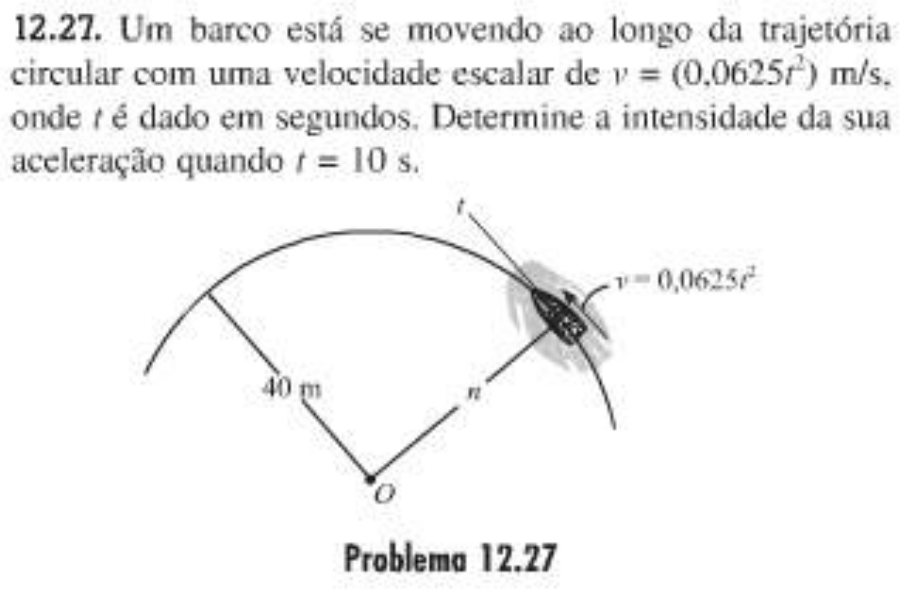
\includegraphics[width=.7\linewidth]{fundamentais/12-27.png}
	\caption{Comando da questão 12-27.}\label{fig:q12-27}
\end{figure}

Nesta questão, analisamos o movimento de uma partícula em uma trajetória circular de raio \(r = 40 \, \text{m}\), cuja velocidade escalar é dada por \(v(t) = 0.0625 \cdot t^2\) (em m/s). Calculamos as acelerações tangencial, centrípeta e total (resultante) e avaliamos seus valores no instante \(t = 10 \, \text{s}\).

\subsection*{Aceleração Tangencial}
A aceleração tangencial é obtida como a derivada da velocidade escalar em relação ao tempo:
\[
a_t = \frac{dv}{dt}.
\]

Derivando \(v(t) = 0.0625 \cdot t^2\):
\[
a_t = \frac{d}{dt}\left(0.0625 \cdot t^2\right) = 0.125 \cdot t.
\]

\subsection*{Aceleração Centrípeta}
A aceleração centrípeta é dada por:
\[
a_c = \frac{v^2}{r}.
\]

Substituímos \(v(t) = 0.0625 \cdot t^2\) e \(r = 40 \, \text{m}\):
\[
a_c = \frac{\left(0.0625 \cdot t^2\right)^2}{40} = \frac{0.00390625 \cdot t^4}{40} = 0.00009765625 \cdot t^4.
\]

\subsection*{Aceleração Total (Resultante)}
A aceleração total é a soma vetorial das componentes tangencial e centrípeta:
\[
a_{\text{total}} = \sqrt{a_t^2 + a_c^2}.
\]

Substituímos \(a_t = 0.125 \cdot t\) e \(a_c = 0.00009765625 \cdot t^4\):
\[
a_{\text{total}} = \sqrt{\left(0.125 \cdot t\right)^2 + \left(0.00009765625 \cdot t^4\right)^2}.
\]

\subsection*{Cálculos no Instante \(t = 10 \, \text{s}\)}
Substituímos \(t = 10 \, \text{s}\) nas expressões para calcular os valores numéricos:
\begin{itemize}
    \item Aceleração tangencial:
    \[
    a_t = 0.125 \cdot 10 = 1.25 \, \text{m/s}^2.
    \]
    \item Aceleração centrípeta:
    \[
    a_c = 0.00009765625 \cdot 10^4 = 0.9765625 \, \text{m/s}^2.
    \]
    \item Aceleração total:
    \[
    a_{\text{total}} = \sqrt{1.25^2 + 0.9765625^2} \approx 1.5862 \, \text{m/s}^2.
    \]
\end{itemize}

